\documentclass[a4paper]{article}
\usepackage[utf8]{inputenc}
\usepackage[margin=1.00in]{geometry}
\usepackage{amsmath}
\usepackage{graphicx}
\usepackage{amsfonts}
\usepackage{listings}
\usepackage{multirow}
\usepackage{tabularx}
\usepackage{hyperref}
\usepackage{fancyhdr}
\usepackage{authblk}
\usepackage[T1]{fontenc}
\usepackage{ascii}
\usepackage{subcaption}
\usepackage[absolute]{textpos}
\usepackage{color}
\usepackage{float}

\pagestyle{fancy}
\fancyhf{}
\fancyfoot[CE,CO]{Juan Pablo Capurro}
\fancyfoot[LE,RO]{\thepage}
\lstset{showstringspaces=false}
\floatstyle{plain} % optionally change the style of the new float
\newfloat{Code}{H}{myc}
\lstloadlanguages{make, C}
\lstset{basicstyle=\ttfamily\footnotesize}
\definecolor{light-gray}{gray}{0.95}
\newcommand{\code}[1]{\colorbox{light-gray}{\texttt{#1}}}

\begin{document}
\begin{titlepage}
    \begin{center}
        \vspace*{1.5cm}
        \huge
        \textbf{Lab1: x86 }
        \vspace{1.5cm}
        
        \Huge
        \textbf{Juan Pablo Capurro}\\
        \vspace{1cm}
        \LARGE
        98194\\
        
        \vspace{2cm}
        
        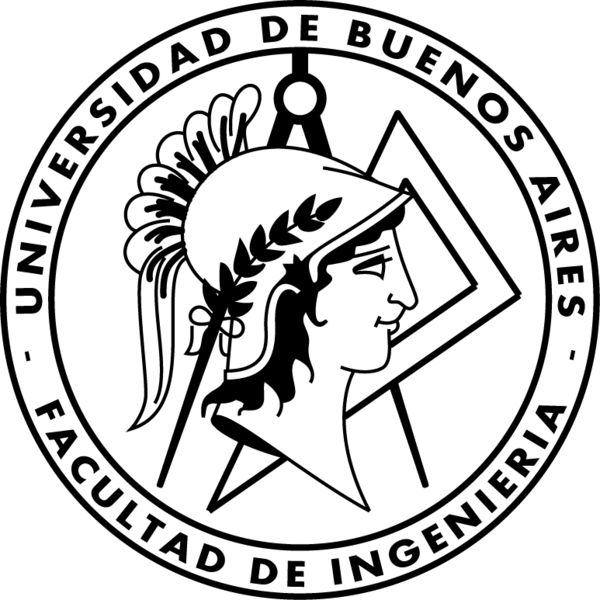
\includegraphics[width=0.4\textwidth]{logo_fiuba.png}
        \vspace{1cm}
        
        07/09/2017\\
        
    \end{center}
\end{titlepage}

\section{Llamadas a biblioteca y llamadas a sistema}
\subsection{Ej: x86-write}
    \subsubsection{¿Por qué se le resta 1 al resultado de sizeof?}
        Es necesario restar \code{1} al resultado de \code{sizeof} porque definir de esa forma a \code{msg} le agrega un byte \code{'\0'} al final del string.
    \subsubsection{¿Funcionaría el programa si se declarase msg como const char *msg = "...";? ¿Por qué?}
        El programa no funciona correctamente ya que el operador \code{sizeof} devuelve 4, el tamaño del puntero \code{msg}, y no el tamaño de memoria alojada al contenido al que apunta.
    \subsubsection{¿Por qué razón se puede escribir sizeof msg en lugar de sizeof(msg)?}
        Eso es posible debido a que \code{sizeof} es un operador y no una función.
    \subsubsection{Explicar el efecto del operador . en la línea \code{.set len, . - msg.}}
        \code{.set} hace que el símbolo \code{len} tenga el valor de la expresión después de la coma, y \code{.} guarda la dirección de la instrucción actual, entonces \code{. - msg} guarda la diferencia entre la dirección actual y el tag \code{msg}, lo que resulta ser el largo del string.
    \subsubsection{Cambiar la directiva .ascii por .asciz y mostrar cómo habría que reescribir la línea \code{push \$len} para que el código siga siendo correcto. (Nota: no cambiar la definición de len.)}
        \code{push \$len -1}
\subsection{Ej: x86-call}
    \subsubsection{Mostrar en una sesión de GDB cómo imprimir las mismas instrucciones usando la directiva \code{x \$pc }y el modificador adecuado. Después, usar el comando \code{stepi} para avanzar la ejecución hasta la llamada a \code{write}. En ese momento, mostrar los primeros cuatro valores de la pila justo antes e inmediatamente después de ejecutar la instrucción \code{call}, y explicar cada uno de ellos.}
        

\subsection{Ej: x86-libc}
\subsection{Ej: x86-ret}
\subsection{Ej: x86-watch}
\section{Stack frames y calling conventions}
\subsection{Ej: x86-ebp}
\subsection{Ej: x86-errno}
\subsection{Ej: x86-argv}
\subsection{Ej: x86-frames}
\subsection{Ej: x86-dwarf}
\section{Creación de stacks en el kernel}
\subsection{Ej: kern1-stack}
\subsection{Ej: kern1-cmdline}
\subsection{Ej: kern1-meminfo}

\end{document}

